\documentclass[english]{article}
\usepackage{float}
\usepackage{graphicx}
\usepackage{needspace}
\usepackage{array}
\usepackage{varwidth}
\usepackage{caption}
\usepackage{babel}
\usepackage[paperwidth=20cm,paperheight=28cm,bottom=5em,top=5em]{geometry}
\usepackage[autostyle]{csquotes}
\usepackage{ragged2e}
\makeatother


\begin{document}
\pagestyle{empty}

%-------------------------------------------------
%	COVER PAGE
%-------------------------------------------------

\begin{center}
\textbf{\large A}{\LARGE{} }
\end{center}
%\vspace{2pt}44444
\begin{center}
\textbf{\LARGE MINI PROJECT PROPOSAL}{\LARGE{} }
\end{center}

\begin{center}
\textbf{\large on}
\end{center}

\begin{center}
\textbf{\Large Web Based platform for pre-ordering food at various food outlets}
\end{center}

\vspace{2pt}
\begin{center}
{\textbf{\large for} } 
\end{center}

\begin{center}
\textbf{\Large T.Y. in Computer Science and Engineering}
\end{center}

\begin{center}
{ \textbf{\large Submitted to}} 
\end{center}
\vspace{2pt}
\begin{figure}[H]
\centering

\includegraphics[scale=0.8]{logo.jpeg}
\end{figure}

\vspace{2pt}
\begin{center}
\textbf{\Large Department of Computer Science and Engineering,}\\
\vspace{5pt}
\textbf{ \large Annasaheb Dange College of Engineering \& Technology,}\\
\vspace{8pt}
\textbf{ \large Ashta, Sangli.}
\end{center}{\Large \par}
\begin{center}
\textbf{(An Autonomous Institute Affiliated to Shivaji University Kolhapur)}
\end{center}

\vspace{2pt}

\begin{center}
{\textbf{by}} 
\end{center}

\begin{center}
\textbf{\large Mr. Rohit Gawas}
\end{center}
\begin{center}
\textbf{\large Mr. Shivam Nimbalkar}
\end{center}
\begin{center}
\textbf{\large Mr. Aditya Vyavahare}
\end{center}
\begin{center}
\textbf{\large Mr. Aryan Magdum}
\end{center}

\vspace{10pt}

\begin{center}
{ \textbf{Under the Guidance of}} 
\end{center}

\begin{center}
\textbf{\Large Asst. Prof. Vishal Kamble}
\end{center}

\vspace{25pt}
\begin{center}
{\large \textbf{Academic Year}} 
\end{center}

\begin{center}
\textbf{\Large 2021-22}
\end{center}

\clearpage % Start a new page


%---------------------------------------------
%	ABSTRACT
%---------------------------------------------



%\begin{center}
\textbf{\Large Abstract}
%\end{center}
\vspace{20pt}
\pagenumbering{roman}

\addcontentsline{toc}{section}{\numberline{}Abstract}%
%\abstract{\addtocontents{toc}{\vspace{1em}} % Add a gap in the Contents, for aesthetics

A fast food restaurant also known as quick service restaurant (QSR) within the food service industry is a specific type of restaurant characterized both by its fast food cuisine
and by minimal table service. Food served in fast food restaurants is offered from a limited
menu, cooked in bulk in advance and kept hot, is finished and packaged for order and is
usually available ready for pickup or to be delivered though seating may also be provided.\\

The customers presently spend an average of 60 minutes per day going to the restaurant,
selecting their meals and paying. Some restaurants have the provision of customers making
a call to the restaurant in advance to order a meal to be ready for them for pick or to be
delivered to them.\\

Some of the customers don’t always get the selection they want because the restaurants run out of certain items or because there is no provision of ordering custom meals. This project
is aimed at developing a complete online ordering system for use in the food service industry
which will allow the restaurants to quickly and easily manage an online menu which customer
can browse and use to place orders with just a few clicks. The customers will have to choose
whether they want the food to be delivered to them or it will be packaged for pick up and
the payment method will be upon delivery or pick up. There will be a system administrator
who will have the right to add and manage user accounts, a manager who will be managing
product and orders and last but not least a meal deliverer who will be dealing specifically
with pending deliveries. The customer will be in a position to view the products,register
and place an order. There will be a confirmation receipt for each and every order made by
the customer which can be printed.\\

The development of this system will be based on CSS and HTML as the programming
languages while local database as the database of the system. HTML language is advantageous
due to its easy to use and learn validation properties while Mongo db has better advanced
features and properties, has good security, is open source and has cross platform operability.\\

\emph {Keywords:} Food Ordering, Pre-Order Restaurant.

\clearpage % Start a new page

\tableofcontents

\pagenumbering{arabic}

\clearpage % Start a new page

\section{Introduction} % creates a section

	Computers have become part of the life for accessing almost any kind of information. Life
in the 21st century is full of technological advancement and in this technological age it is
very difficult for any organization to survive without utilizing technology. The World Wide
Web contributes greatly to the creation of an ever-increasing global information database.
It could also be used as a mechanism to share information within an enterprise.

In today’s age of fast food and take-out, many restaurants have chosen to focus on quick
preparation, offering a rich dining experience. Until very recently, all of these, but there
are many disadvantages to this system, including the inconvenience of the customer needing
to have a physical copy of the menu, lack of a visual confirmation that the order was placed
correctly, and the necessity for the restaurant to have an employee answering the phone and
taking orders.



\subsection{Background and Context}
It will lighten the load on the restaurant’s end to a much greater extent, as the entire process
of taking orders is automated. Once an order is placed on the webpage, it is entered into
the database and then retrieved, in pretty much real-time, by a desktop application on the
restaurant’s end. Within this application, all items in the order will be displayed, along with
their corresponding options, in a concise and easy to read manner. This allows restaurant
employees to quickly go through the orders as they are placed and produce the necessary
items with minimal delay and confusion.

\subsection{Purpose}
To increase efficiency and improve services provided to the customers in the restaurant
through better application of technology in daily operations.


\section{Literature Survey} % creates a section


In the paper by Bhandge. K, et al [1.] The advancement in information and communication
technology has greatly influenced the business transactions. In
earlier days, food industry traditionally has lagged behind other
industries in adopting new technology. However rapid advances
in computer Technology and heightened expectations of
consumers have forced the food industry to bring automation in
the process. Nowadays, the adoption of wireless technology and
emergence of mobile devices has led to automation in the food
industry. The business and services in restaurants can be
improved with the combination of wireless and mobile
technologies. The competition in restaurants with respect to
business has increased with the advancements in food ordering
techniques .\\

According to the work of Bhargave A., et al [2.], nowadays web services technology is widely used to integrate
heterogeneous systems and develop new applications. Here an
application of integration of hotel management systems by web
services technology is presented. Digital Hotel Management
integrates lots of systems of hotel industry such as Ordering
System Kitchen Order Ticket (KOT), Billing System, Customer
Relationship Management system (CRM) together. This
integration solution can add or expand hotel software system in
any size of hotel chains environment. This system increases
quality and speed of service. This system also increases attraction
of place for large range of customers. Implementing this system
gives a cost-efficient opportunity to give your customers a
personalized service experience where they are in control
choosing what they want, when they want it – from dining to
ordering to payment and feedback .\\

\clearpage % Start a new page
By Patel Krishna, et al [3.], the research work aims to automate the food
ordering process in restaurant and also improve the dining
experience of customers. Design implementation of food
ordering system for restaurants were discuss in this paper.
This system implements wireless data access to servers. The
android application on user’s mobile will have all the menu
details. Kitchen and cashier receives the order details from
the customer mobile wirelessly. These order details are
updated in the central database. The restaurant owner can
manage the menu modifications easily.\\

In the paper by Shinde R., et al [4.] there was an attempt to design and implementation
of digital dining in restaurants using android technology.
This system was a basic dynamic database utility system
which fetches all information from a centralized database.
This application improved the accuracy and efficiency of
restaurants as well as human errors. Earlier drawbacks of
automated food ordering systems were overcome by this
system and it requires a onetime investment for gadgets.\\


 According to the work of Mayur, et al [5.] he
proposed the low cost touch screen based Restaurant
Management System using an android Smartphone or tablet as a
solution against the conventional paper based and Personal
Digital Assistant (PDA) based food ordering system. The system
consists of a Smartphone/tablet at the customer table contains the
android application with all the menu details. The customer
tablet, kitchen display connects directly with each other through
Wi-Fi. Orders made by the customers will be instantly reach the
kitchen module. This wireless application is user-friendly,
improves efficiency and accuracy for restaurants by saving time,
reduces human errors and provides customer feedback. This
system successfully overcomes the drawbacks in earlier
automated food ordering systems and is less expensive as it
requires a one-time investment for gadgets. \\ \\ Table 1 shows the Comparison of the selected approaches


\begin{table}[ht]
\centering
% To place a caption above a table

\begin{tabular}{ ||c|c|c| } \hline
\centering
% To place a caption above a table

\textbf{Paper/year} &  \textbf{Approach Used} &\textbf{Limitations} 
                   \\  \hline
[1]/2015  & Java for software development   &  Cannot accept different types of , \\
 & JSP/SERVLET is used for  & payments methods like \\  
 &  Remote Database Access. &credit cards, debit cards\\  
 & SQLite for BackEnd &\\ \hline 
[2]/2015  & HTML, CSS, JavaScript & Cannot register and link multiple \\
 & &restaurants to enhance\\
&& the dining experience of customers. \\ \hline 
[3]/2015  & Android Application  & Gadgets are costlier, \\
&& regular maintenance is needed, \\ \hline

[4]/2015  & Android Application  & Technical assistance would be needed. \\ \hline 

[5]/2015 &Android Application & Conventional paper based \\
  &  &and PDA-based food ordering system,\\
  & &proposed the low-cost touch \\
  & &screen-based Restaurant Management System \\ \hline 
\end{tabular} \\
\caption{Comparison of selected approaches}
\end{table}%

\clearpage % Start a new page
\section{Problem Statement} % creates a section
\begin{itemize}
\item IDEAL: Fast food business in a very competitive business
and one way to stand out from competitors is through improving the business process where
business process automation can assist business improvement. The customer will be able to order the food conveniently and pay efficiently via online transaction.
\item REALITY: The challenges encountered by the existing system serve as a major drawback to the realization of efficiency and customer satisfaction. Gadgets are costlier, Technical assistance is needed regularly. The other problem with the
current system is that the customers are not able to see the ingredients of the meals.
\item  CONSEQUENCES: If the problem is not fixed or improved food industry will be impacted with the loss in productivity, profits.
\end{itemize}
\section{Objectives} % creates a section
\begin{itemize}

\item[1.] To create an interactive UI. 

\item[2.] To design and create database .

\item[3.] To Design registration form, login form, Dashboard, form for getting food orders.

\item[4.] To Establish connection between frontend and backend of the system.

\item[5.] To Test the entire system.

\end{itemize}

\section{Scope} % creates a section

\begin{itemize}
\item Requires internet connection and also the user must be computer literate.
\item The set back of the system is that the customers targeted are adults with access to
computer systems / Mobile Devices while the minors might have to go physically to
the restaurant to purchase the food that they want or order food the food with the
help of an adult.
\item The other limitation is that the system will only be convenient to people with a small
geographical region, basically just around the restaurant i.e. can only help a small area.
\end{itemize}
\section{Proposed Work} % creates a section
\subsection{Methodology}
\begin{itemize}
\item Development of computerized systems requires analysis of the process to be digitized
inorder to enable a correct system, a system that functions as required and to assist
the potential users of the system understand the general functionality of the system.
The analysis specifies the system’s objectives and constraints to which designers have
to comply. The purpose of doing analysis is to transform the system’s major inputs
into structured specification.
\item This is a brief structure which depicts the environment in which a software system
exists and helps in communicating about what lies outside the system boundary.
\item Figure 1 shows how the data will flow into the system.
\begin{figure}[H]
\centering
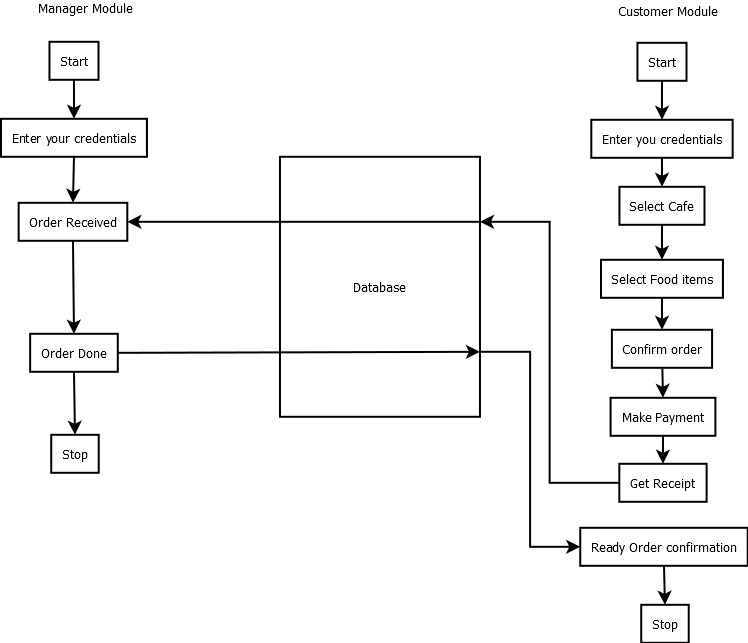
\includegraphics[scale=0.4]{map.jpeg}
\caption{ A Block Diagram showing order management}
\end{figure}
It is a two-dimensional diagram that explains how data is processed and transferred
in a system. The graphical depiction identifies each source of data and how it interacts
with other data sources to reach a common output.

Figure 2 shows the ER diagram of the system
\begin{figure}[H]
\centering
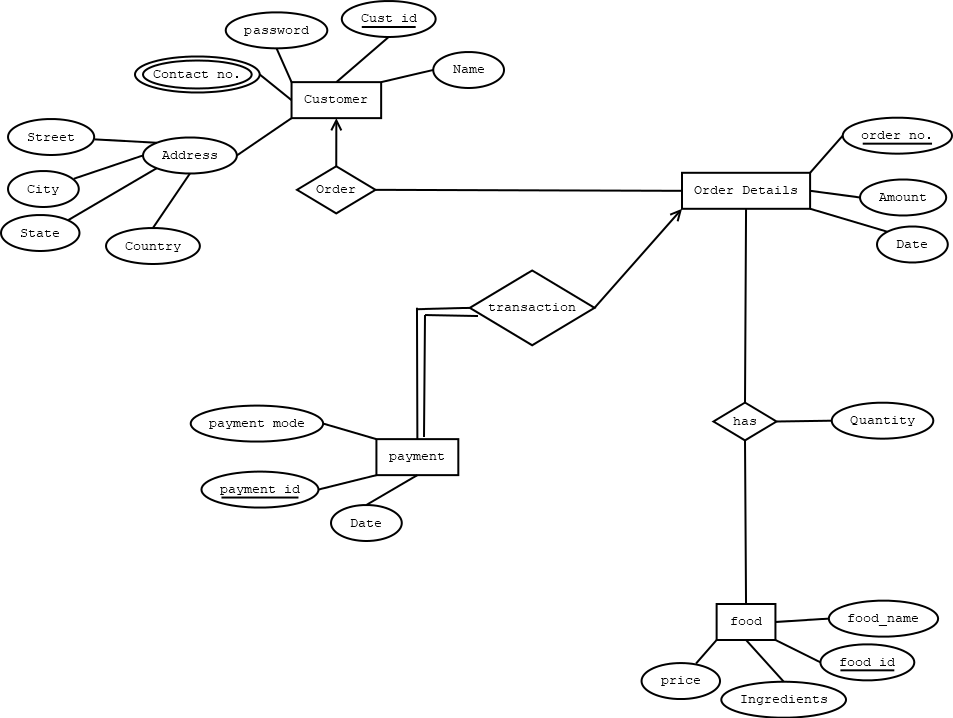
\includegraphics[scale=0.4]{ER.png}
\caption{Project ER diagram}
\end{figure}


\clearpage % Start a new page
The simulation first starts with the customer entering
his/her credentials (name, ID and password). Once that has
been verified, the customer can place an order specifying the
quantity of the food required. Now we get a window that
displays the order number, customer ID, food name, price
and quantity. Once the customer finalizes his/her order, they
are redirected to the payment window where the total price
is displayed and the customer can select the payment
method of their choice and then the customer gets a message
of confirmation of order. \\

The above mentioned simulation flow is with respect to
the customer's point of view. Now if you are an admin, you
can select the normal login option and enter the admin
credentials (email ID and password). Once you enter the
admin portal, you get the option of adding food, deleting
food or updating food. Any option of choice leads you to the
food menu. Once the selected operation is carried out, the
end result, i.e, the added food or the updated food list is
displayed and if you have deleted a food, that particular food
disappears from the main menu.\\

Functionalities provided:
\item Create usernames and passwords
\item View user / admin accounts

Customer module:
\item Add items to cart
\item View final checkout cart
\item Confirm order and proceed for payment

Manager module:
\item Create product categories and functionalities
\item Edit / delete product categories and descriptions

\end{itemize}
\subsection{Software and Hardware requirements and availability}
\begin{itemize}
\subsubsection {Software Requirement}
\item Operating system: Win 7 / Win 8 / Win 10 / Win 11 / macOS 10 and later
\item Technology : HTML, CSS, PHP
\item Database : MySQL
\item Antivirus software

\subsubsection {Hardware Requirement}
\item Processor: Intel dual core and above
\item Processor Speed: 1.0GHZ and above
\item RAM: 1 GB RAM and above
\item Hard Disk: 20 GB hard disk and above
\item Printer for printing reports
\item  Uninterruptible power supply

\end{itemize}
\section{Schedule} % creates a section

\begin{itemize}
\item Split entire work into subtasks such as literature survey, planning, development, installation, testing, writing reports or articles

\item Prepare Gantt Chart
\end{itemize}

Figure 3 shows the project schedule to be used to implement the project.

\begin{figure}[H]
\centering
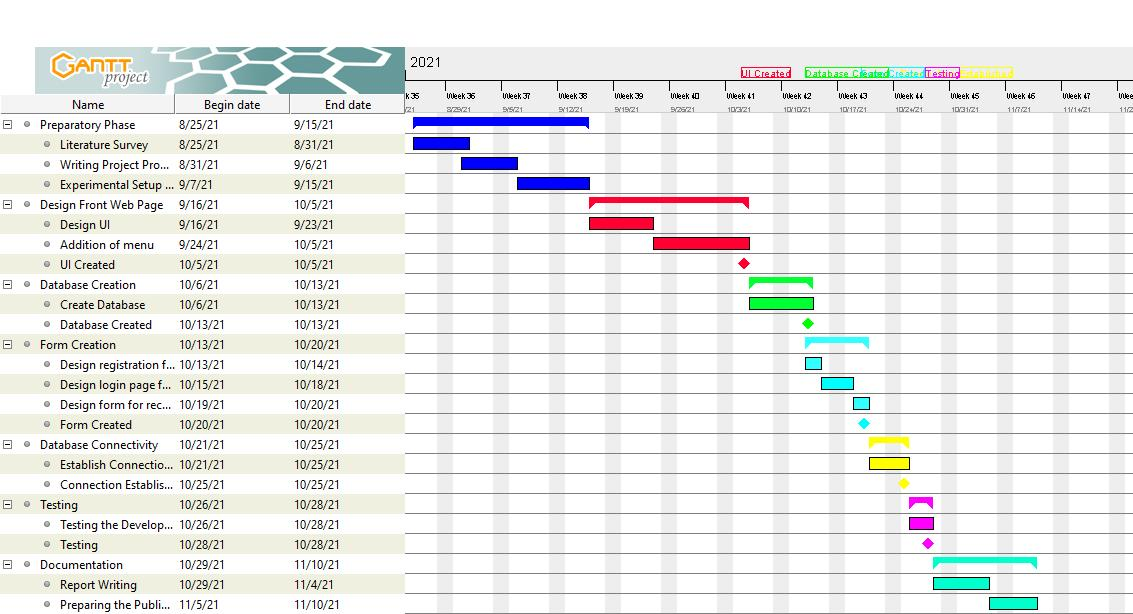
\includegraphics[scale=0.4]{schedule.jpg}
\caption{Project Schedule}
\end{figure}


\addcontentsline{toc}{section}{References}

\section*{References}
\vspace{20pt}


\begin{itemize}
\item[[1]] Bhandge. K, Shinde. T, Ingale .D, Solanki .N, Totare .R, 2015 \emph{"A Proposed
System for Touchpad Based Food Ordering System Using Android
Application"}, International Journal  of Advanced Research in Computer
Science Technology (IJARCST) 2015.

\item [[2]] Bhargave A., Jadhav N, Joshi A., Oke. P, Lahane S. R, 2013 \emph{"Digital
Ordering System for Restaurant Using Android"}, International Journal of
Scientific and Research Publications, Volume 3, Issue 4, 1 ISSN 2250-3153
\item [[3]] Patel Krishna, Patel Palak, Raj Nirali, Patel Lalit,\emph{”Automated Food Ordering System”}, International Journal of
Engineering Research and Development (IJERD) 2015.
\item [[4]] Shinde R., Thakare P., Dhomne N. and Sarkar S., 2014 \emph{"Design and
Implementation of Digital dining in Restaurants using Android"},
International Journal of Advance Research in Computer Science and
Management Studies. Volume 2, Issue 1.
\item [[5]] Mayur D. Jakhete, Piyush C. Mankar, \emph{”Implementation of
Smart Restaurant with e-menu Card"}, International Journal
of Computer Applications 2015 of Smart Restaurant with e-menu Card, International Journal of Computer Applications
2015.

\end{itemize}
\vspace{20pt}

\section*{Group Members}
\vspace{20pt}

\centering
\begin{tabular}{ | c | c | c | c | c | c |}
     
\hline \bf{Sr.NO} &\textbf{Name of the Student} &\textbf{Contact No.} &\textbf{Email ID} 
&\textbf{Signature}  \\ 
     \hline    1& Rohit Gawas &8839867653 &19131084\_cse@adcet.in &\\ 
     \hline    2 &Shivam Nimbalkar &8830854483 & 19131035\_cse@adcet.in&\\ 
     \hline    3& Aditya Vyavahare& 9561648317&19131076\_cse@adcet.in &    \\
     \hline  4 &Aryan Magdum & 8308992976&19131079\_cse@adcet.in & \\ 

     \hline
    
      
\end{tabular}


\vspace{20pt}

\begin{FlushLeft}
Date: \today 
\\
\vspace{20pt}
Place: Ashta
\end{FlushLeft}
\vspace{20pt}
\textbf{Mr.Vishal Kamble} \hspace{13pc} \textbf{Mrs. Ashwini Patil}  \ \ \ \quad 
\\
\textbf{GUIDE}     \hspace{16pc}    \textbf{Project Coordinator}\ \ \ \ \quad 
\\
\vspace{30pt}
\begin{center}
\textbf{Dr. Srmiti H. Bhandari} \ \ \ \quad 
\\
\textbf{HoD, CSE} \ \ \ \quad 

\end{center}


\clearpage % Start a new page



\end{document}